% fig07_subaxis_falsifiers — preregistered falsifier count per UFO sub-axis.
% Standalone pgfplots; compiled to figures/fig07_subaxis_falsifiers.pdf.
% Comparison (falsifier count across sub-axes) => chart (user hard rule).
% Data: Appendix E, UFO/{grav,cloak,hexa-teleport}/*.md.
%   HEXA-GRAV 4, HEXA-CLOAK 4, HEXA-TELEPORT 1, HEXA-HOVER 0, HEXA-SIM 0.
\documentclass[border=4pt]{standalone}
\usepackage{tikz}
\usepackage{pgfplots}
\pgfplotsset{compat=1.18}
\begin{document}
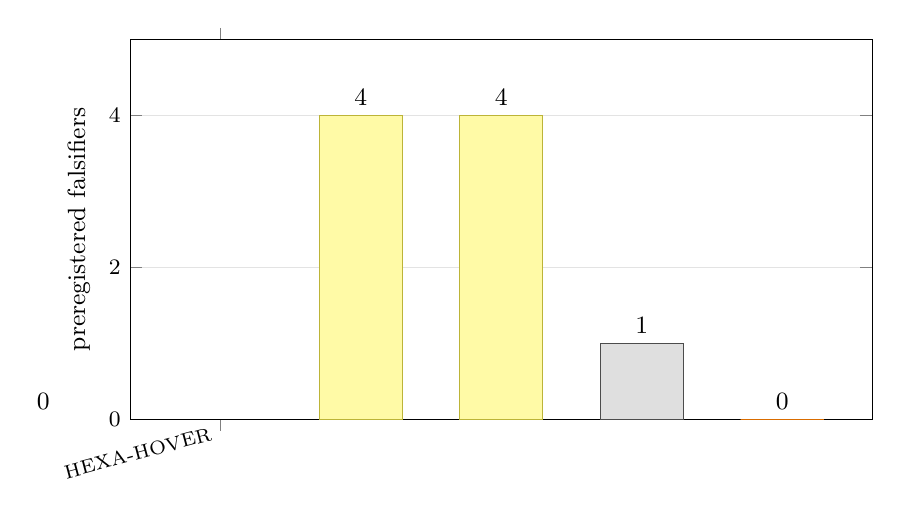
\begin{tikzpicture}
\begin{axis}[
  width=11cm, height=6.4cm,
  ybar,
  bar width=30pt,
  ymin=0, ymax=5,
  ylabel={preregistered falsifiers},
  symbolic x coords={HEXA-HOVER, HEXA-GRAV, HEXA-CLOAK, HEXA-TELEPORT, HEXA-SIM},
  xtick=data,
  x tick label style={font=\scriptsize, rotate=15, anchor=east},
  tick label style={font=\footnotesize},
  label style={font=\small},
  nodes near coords,
  nodes near coords style={font=\small},
  ymajorgrids, grid style={gray!22},
  enlarge x limits=0.16,
]
\addplot[draw=green!55!black,fill=green!30] coordinates {(HEXA-HOVER,0)};
\addplot[draw=yellow!70!black,fill=yellow!35, bar shift=0pt] coordinates {(HEXA-GRAV,4)};
\addplot[draw=yellow!70!black,fill=yellow!35, bar shift=0pt] coordinates {(HEXA-CLOAK,4)};
\addplot[draw=gray!60!black,fill=gray!25, bar shift=0pt] coordinates {(HEXA-TELEPORT,1)};
\addplot[draw=orange!85!black,fill=orange!30, bar shift=0pt] coordinates {(HEXA-SIM,0)};
\end{axis}
\end{tikzpicture}
\end{document}
